\subsection{问题一：确定性日循环购电}
\subsubsection{模型求解与最优性核验}
在附件一预测确定时，令$e_t=0,q_t=g_t$，施加$S_0=S_{144}=6000$，求解
\begin{equation}
 \min \sum_{t=0}^{143}p_tg_t
 \quad\text{s.t. 式\eqref{eq:balance}--\eqref{eq:nonnegative}的线性约束及日循环边界。}
\end{equation}
依据前述等价论证，求解时去掉互斥乘积约束。以购电、充电、放电、段末储电量和未利用量为变量，共有720个连续变量与288个线性等式。经SciPy的HiGHS接口求解\upcite{scipyHighs}；对偶修正单纯形算法已有详细论述\upcite{huangfu2018simplex}。数值计算以微小吞吐项$10^{-6}\sum_t(c_t+b_t)+10^{-7}\sum_tw_t$选择退化解，但报告费用不包含这些选解项。

不加选解项的纯电费LP给出相同费用；另引入144个充放电模式二元变量，独立求解MILP，所得费用亦为35126.948589元，最优性间隙为0，最大约束残差约$7.62\times10^{-12}$。故最优性结论适用于给定离散化、效率和余电处理假设下的问题一。

\subsubsection{指定时段结果与储能作用}
表\ref{tab:q1-purchase}给出六个指定区间及全天购电结果，表\ref{tab:q1-storage}按六个连续四小时区间汇总交流母线侧的充电输入与放电输出，末行分别列出00:00和24:00的储电量。这样既能核对日循环边界，也能区分能量损耗前后的充、放电量。
% Generated by scripts/build_paper_tables.py; do not edit by hand.
\par
\begin{table}[!htbp]
\centering
\caption{微网在指定时间段的购电量及全天的购电量和购电费}\label{tab:q1-purchase}
\normalsize
\begin{tabular}{lrlrlr}
\toprule
\multicolumn{1}{c}{时间段} & \multicolumn{1}{c}{购电量} & \multicolumn{1}{c}{时间段} & \multicolumn{1}{c}{购电量} & \multicolumn{1}{c}{时间段} & \multicolumn{1}{c}{购电量} \\
\midrule
10:00--10:10 & 0.00 & 12:00--12:10 & 480.41 & 14:00--14:10 & 0.00 \\
16:00--16:10 & 445.43 & 18:00--18:10 & 531.89 & 20:00--20:10 & 0.00 \\
\multicolumn{2}{c}{全天购电量} & 59,482.70 & \multicolumn{2}{c}{全天购电费} & 35,126.95 \\
\bottomrule
\end{tabular}
\end{table}
\par

\par
\begin{table}[!htbp]
\centering
\caption{储能设备在指定时间段的充放电量及0:00和24:00的储电量}\label{tab:q1-storage}
\normalsize
\begin{tabular}{lrrlrr}
\toprule
\multicolumn{1}{c}{时间段} & \multicolumn{1}{c}{充电量} & \multicolumn{1}{c}{放电量} & \multicolumn{1}{c}{时间段} & \multicolumn{1}{c}{充电量} & \multicolumn{1}{c}{放电量} \\
\midrule
0:00--4:00 & 4,500.00 & 0.00 & 4:00--8:00 & 833.33 & 6,365.84 \\
8:00--12:00 & 4,787.96 & 1,703.00 & 12:00--16:00 & 5,286.04 & 91.10 \\
16:00--20:00 & 0.00 & 5,780.13 & 20:00--24:00 & 5,333.33 & 2,859.87 \\
\multicolumn{2}{c}{0:00储电量} & 6,000.00 & \multicolumn{2}{c}{24:00储电量} & 6,000.00 \\
\bottomrule
\end{tabular}
\end{table}
\par

\begin{figure}[htbp]
  \centering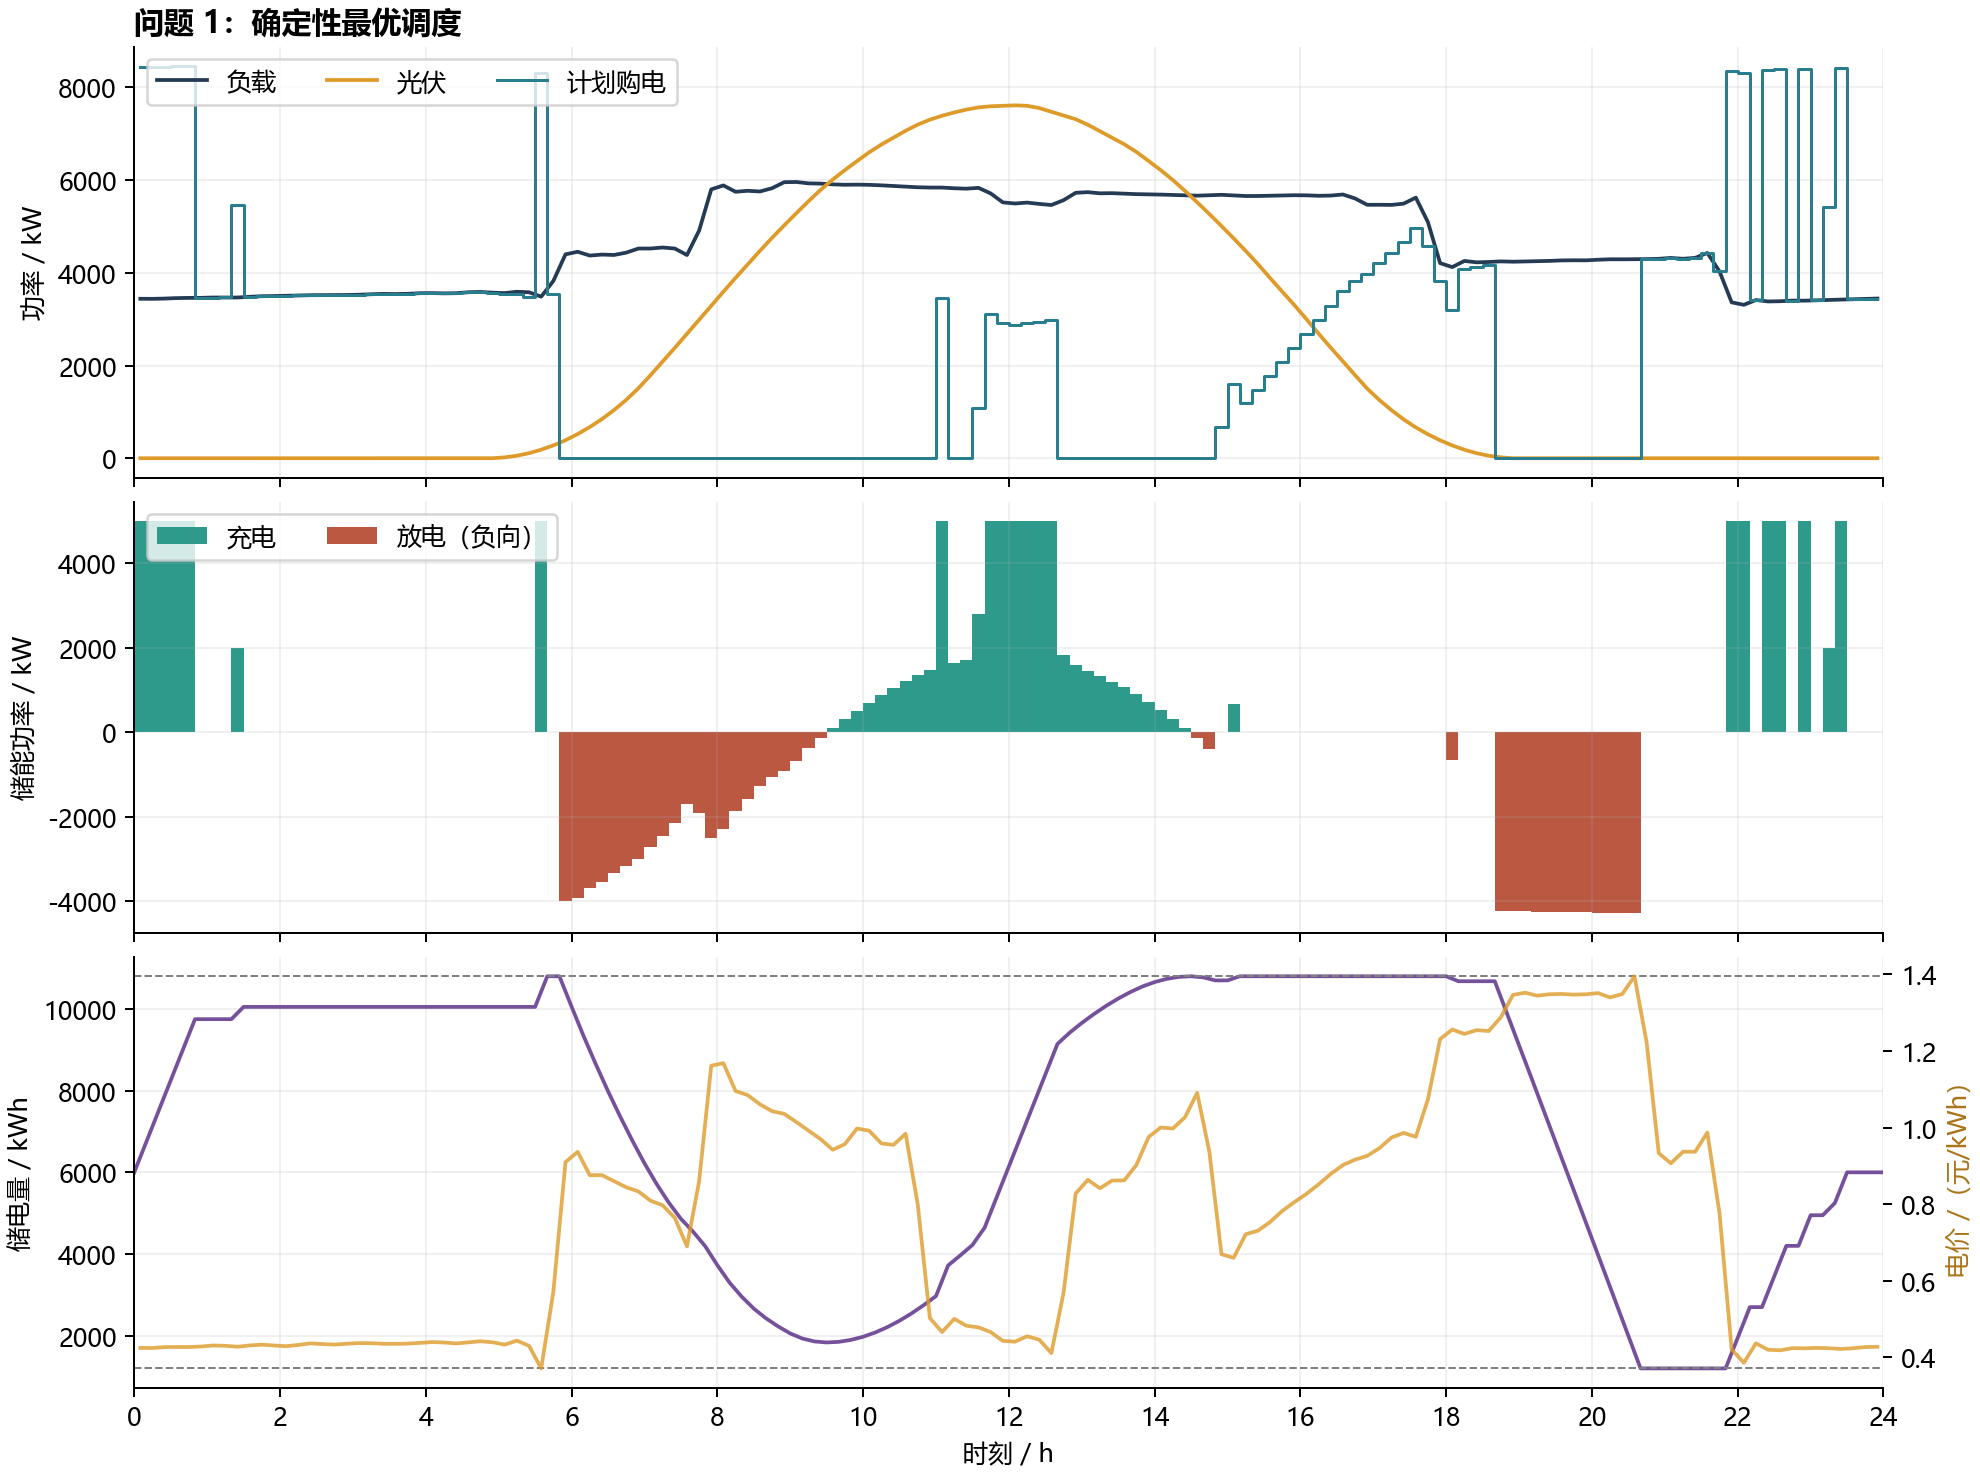
\includegraphics[width=\textwidth]{../outputs/figures/q1-dispatch.png}
  \caption{问题一的最优购电与储能调度}\label{fig:q1}
\end{figure}
在低电价或光伏富余区间储能，可在高电价时替代购电。但每向电池输入1\,kWh，只能最终向母线输出0.81\,kWh；仅考虑套利时，放电段替代电价至少要高于充电段电价除以0.81。容量和功率约束进一步限制了负荷可以转移的数量。表中某个四小时区间内充电总量与放电总量同时为正，并不意味着某个十分钟段同时充放电。
\FloatBarrier
